\documentclass[1p]{elsarticle_modified}
%\bibliographystyle{elsarticle-num}

%\usepackage[colorlinks]{hyperref}
%\usepackage{abbrmath_seonhwa} %\Abb, \Ascr, \Acal ,\Abf, \Afrak
\usepackage{amsfonts}
\usepackage{amssymb}
\usepackage{amsmath}
\usepackage{amsthm}
\usepackage{scalefnt}
\usepackage{amsbsy}
\usepackage{kotex}
\usepackage{caption}
\usepackage{subfig}
\usepackage{color}
\usepackage{graphicx}
\usepackage{xcolor} %% white, black, red, green, blue, cyan, magenta, yellow
\usepackage{float}
\usepackage{setspace}
\usepackage{hyperref}

\usepackage{tikz}
\usetikzlibrary{arrows}

\usepackage{multirow}
\usepackage{array} % fixed length table
\usepackage{hhline}

%%%%%%%%%%%%%%%%%%%%%
\makeatletter
\renewcommand*\env@matrix[1][\arraystretch]{%
	\edef\arraystretch{#1}%
	\hskip -\arraycolsep
	\let\@ifnextchar\new@ifnextchar
	\array{*\c@MaxMatrixCols c}}
\makeatother %https://tex.stackexchange.com/questions/14071/how-can-i-increase-the-line-spacing-in-a-matrix
%%%%%%%%%%%%%%%

\usepackage[normalem]{ulem}

\newcommand{\msout}[1]{\ifmmode\text{\sout{\ensuremath{#1}}}\else\sout{#1}\fi}
%SOURCE: \msout is \stkout macro in https://tex.stackexchange.com/questions/20609/strikeout-in-math-mode

\newcommand{\cancel}[1]{
	\ifmmode
	{\color{red}\msout{#1}}
	\else
	{\color{red}\sout{#1}}
	\fi
}

\newcommand{\add}[1]{
	{\color{blue}\uwave{#1}}
}

\newcommand{\replace}[2]{
	\ifmmode
	{\color{red}\msout{#1}}{\color{blue}\uwave{#2}}
	\else
	{\color{red}\sout{#1}}{\color{blue}\uwave{#2}}
	\fi
}

\newcommand{\Sol}{\mathcal{S}} %segment
\newcommand{\D}{D} %diagram
\newcommand{\A}{\mathcal{A}} %arc


%%%%%%%%%%%%%%%%%%%%%%%%%%%%%5 test

\def\sl{\operatorname{\textup{SL}}(2,\Cbb)}
\def\psl{\operatorname{\textup{PSL}}(2,\Cbb)}
\def\quan{\mkern 1mu \triangleright \mkern 1mu}

\theoremstyle{definition}
\newtheorem{thm}{Theorem}[section]
\newtheorem{prop}[thm]{Proposition}
\newtheorem{lem}[thm]{Lemma}
\newtheorem{ques}[thm]{Question}
\newtheorem{cor}[thm]{Corollary}
\newtheorem{defn}[thm]{Definition}
\newtheorem{exam}[thm]{Example}
\newtheorem{rmk}[thm]{Remark}
\newtheorem{alg}[thm]{Algorithm}

\newcommand{\I}{\sqrt{-1}}
\begin{document}

%\begin{frontmatter}
%
%\title{Boundary parabolic representations of knots up to 8 crossings}
%
%%% Group authors per affiliation:
%\author{Yunhi Cho} 
%\address{Department of Mathematics, University of Seoul, Seoul, Korea}
%\ead{yhcho@uos.ac.kr}
%
%
%\author{Seonhwa Kim} %\fnref{s_kim}}
%\address{Center for Geometry and Physics, Institute for Basic Science, Pohang, 37673, Korea}
%\ead{ryeona17@ibs.re.kr}
%
%\author{Hyuk Kim}
%\address{Department of Mathematical Sciences, Seoul National University, Seoul 08826, Korea}
%\ead{hyukkim@snu.ac.kr}
%
%\author{Seokbeom Yoon}
%\address{Department of Mathematical Sciences, Seoul National University, Seoul, 08826,  Korea}
%\ead{sbyoon15@snu.ac.kr}
%
%\begin{abstract}
%We find all boundary parabolic representation of knots up to 8 crossings.
%
%\end{abstract}
%\begin{keyword}
%    \MSC[2010] 57M25 
%\end{keyword}
%
%\end{frontmatter}

%\linenumbers
%\tableofcontents
%
\newcommand\colored[1]{\textcolor{white}{\rule[-0.35ex]{0.8em}{1.4ex}}\kern-0.8em\color{red} #1}%
%\newcommand\colored[1]{\textcolor{white}{ #1}\kern-2.17ex	\textcolor{white}{ #1}\kern-1.81ex	\textcolor{white}{ #1}\kern-2.15ex\color{red}#1	}

{\Large $\underline{12n_{0266}~(K12n_{0266})}$}

\setlength{\tabcolsep}{10pt}
\renewcommand{\arraystretch}{1.6}
\vspace{1cm}\begin{tabular}{m{100pt}>{\centering\arraybackslash}m{274pt}}
\multirow{5}{120pt}{
	\centering
	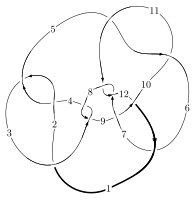
\includegraphics[width=112pt]{../../../GIT/diagram.site/Diagrams/png/2355_12n_0266.png}\\
\ \ \ A knot diagram\footnotemark}&
\allowdisplaybreaks
\textbf{Linearized knot diagam} \\
\cline{2-2}
 &
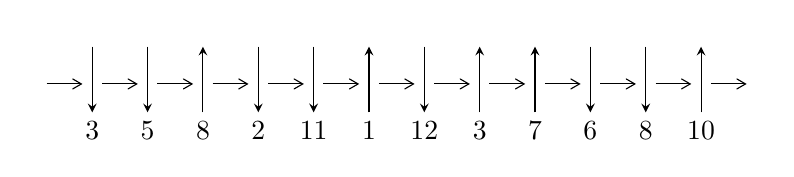
\begin{tikzpicture}[x=20pt, y=17pt]
	% nodes
	\node (C0) at (0, 0) {};
	\node (C1) at (1, 0) {};
	\node (C1U) at (1, +1) {};
	\node (C1D) at (1, -1) {3};

	\node (C2) at (2, 0) {};
	\node (C2U) at (2, +1) {};
	\node (C2D) at (2, -1) {5};

	\node (C3) at (3, 0) {};
	\node (C3U) at (3, +1) {};
	\node (C3D) at (3, -1) {8};

	\node (C4) at (4, 0) {};
	\node (C4U) at (4, +1) {};
	\node (C4D) at (4, -1) {2};

	\node (C5) at (5, 0) {};
	\node (C5U) at (5, +1) {};
	\node (C5D) at (5, -1) {11};

	\node (C6) at (6, 0) {};
	\node (C6U) at (6, +1) {};
	\node (C6D) at (6, -1) {1};

	\node (C7) at (7, 0) {};
	\node (C7U) at (7, +1) {};
	\node (C7D) at (7, -1) {12};

	\node (C8) at (8, 0) {};
	\node (C8U) at (8, +1) {};
	\node (C8D) at (8, -1) {3};

	\node (C9) at (9, 0) {};
	\node (C9U) at (9, +1) {};
	\node (C9D) at (9, -1) {7};

	\node (C10) at (10, 0) {};
	\node (C10U) at (10, +1) {};
	\node (C10D) at (10, -1) {6};

	\node (C11) at (11, 0) {};
	\node (C11U) at (11, +1) {};
	\node (C11D) at (11, -1) {8};

	\node (C12) at (12, 0) {};
	\node (C12U) at (12, +1) {};
	\node (C12D) at (12, -1) {10};
	\node (C13) at (13, 0) {};

	% arrows
	\draw[->,>={angle 60}]
	(C0) edge (C1) (C1) edge (C2) (C2) edge (C3) (C3) edge (C4) (C4) edge (C5) (C5) edge (C6) (C6) edge (C7) (C7) edge (C8) (C8) edge (C9) (C9) edge (C10) (C10) edge (C11) (C11) edge (C12) (C12) edge (C13) ;	\draw[->,>=stealth]
	(C1U) edge (C1D) (C2U) edge (C2D) (C3D) edge (C3U) (C4U) edge (C4D) (C5U) edge (C5D) (C6D) edge (C6U) (C7U) edge (C7D) (C8D) edge (C8U) (C9D) edge (C9U) (C10U) edge (C10D) (C11U) edge (C11D) (C12D) edge (C12U) ;
	\end{tikzpicture} \\
\hhline{~~} \\& 
\textbf{Solving Sequence} \\ \cline{2-2} 
 &
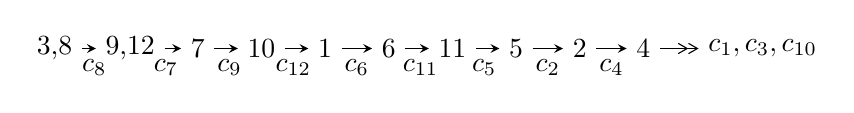
\begin{tikzpicture}[x=23pt, y=7pt]
	% node
	\node (A0) at (-1/8, 0) {3,8};
	\node (A1) at (17/16, 0) {9,12};
	\node (A2) at (17/8, 0) {7};
	\node (A3) at (25/8, 0) {10};
	\node (A4) at (33/8, 0) {1};
	\node (A5) at (41/8, 0) {6};
	\node (A6) at (49/8, 0) {11};
	\node (A7) at (57/8, 0) {5};
	\node (A8) at (65/8, 0) {2};
	\node (A9) at (73/8, 0) {4};
	\node (C1) at (1/2, -1) {$c_{8}$};
	\node (C2) at (13/8, -1) {$c_{7}$};
	\node (C3) at (21/8, -1) {$c_{9}$};
	\node (C4) at (29/8, -1) {$c_{12}$};
	\node (C5) at (37/8, -1) {$c_{6}$};
	\node (C6) at (45/8, -1) {$c_{11}$};
	\node (C7) at (53/8, -1) {$c_{5}$};
	\node (C8) at (61/8, -1) {$c_{2}$};
	\node (C9) at (69/8, -1) {$c_{4}$};
	\node (A10) at (11, 0) {$c_{1},c_{3},c_{10}$};

	% edge
	\draw[->,>=stealth]	
	(A0) edge (A1) (A1) edge (A2) (A2) edge (A3) (A3) edge (A4) (A4) edge (A5) (A5) edge (A6) (A6) edge (A7) (A7) edge (A8) (A8) edge (A9) ;
	\draw[->>,>={angle 60}]	
	(A9) edge (A10);
\end{tikzpicture} \\ 

\end{tabular} \\

\footnotetext{
The image of knot diagram is generated by the software ``\textbf{Draw programme}" developed by Andrew Bartholomew(\url{http://www.layer8.co.uk/maths/draw/index.htm\#Running-draw}), where we modified some parts for our purpose(\url{https://github.com/CATsTAILs/LinksPainter}).
}\phantom \\ \newline 
\centering \textbf{Ideals for irreducible components\footnotemark of $X_{\text{par}}$} 
 
\begin{align*}
I^u_{1}&=\langle 
1.30470\times10^{57} u^{29}-8.04261\times10^{57} u^{28}+\cdots+3.78260\times10^{57} b-1.44716\times10^{60},\\
\phantom{I^u_{1}}&\phantom{= \langle  }1.67303\times10^{56} u^{29}-2.36382\times10^{57} u^{28}+\cdots+3.02608\times10^{58} a-1.98438\times10^{60},\\
\phantom{I^u_{1}}&\phantom{= \langle  }u^{30}-7 u^{29}+\cdots-8960 u+1024\rangle \\
I^u_{2}&=\langle 
85 a^5 u^3+81 a^4 u^3+\cdots-914 a-116,\;4 a^5 u^3+36 a^4 u^3+\cdots+70 a-27,\;u^4+3 u^3+3 u^2+2 u+2\rangle \\
I^u_{3}&=\langle 
4147258 u^{15}+7664206 u^{14}+\cdots+53503381 b+7608876,\\
\phantom{I^u_{3}}&\phantom{= \langle  }-151936201 u^{15}+44795175 u^{14}+\cdots+53503381 a-367339747,\\
\phantom{I^u_{3}}&\phantom{= \langle  }u^{16}-3 u^{14}-4 u^{12}+5 u^{11}+23 u^{10}-7 u^9-13 u^8+6 u^7-11 u^6-12 u^5+13 u^4-4 u^3+5 u^2+u+1\rangle \\
I^u_{4}&=\langle 
9.10023\times10^{19} a^{11} u+1.90099\times10^{20} a^{10} u+\cdots+3.63923\times10^{20} a+7.09845\times10^{19},\\
\phantom{I^u_{4}}&\phantom{= \langle  }- a^{11} u-29 a^{10} u+\cdots-3954 a+1387,\;u^2- u-1\rangle \\
\\
I^v_{1}&=\langle 
a,\;8 v^3+12 v^2+b+10 v+3,\;8 v^4+12 v^3+12 v^2+5 v+1\rangle \\
I^v_{2}&=\langle 
a,\;b^6+b^5+2 b^4+2 b^3+2 b^2+2 b+1,\;v-1\rangle \\
\end{align*}
\raggedright * 6 irreducible components of $\dim_{\mathbb{C}}=0$, with total 104 representations.\\
\footnotetext{All coefficients of polynomials are rational numbers. But the coefficients are sometimes approximated in decimal forms when there is not enough margin.}
\newpage
\renewcommand{\arraystretch}{1}
\centering \section*{I. $I^u_{1}= \langle 1.30\times10^{57} u^{29}-8.04\times10^{57} u^{28}+\cdots+3.78\times10^{57} b-1.45\times10^{60},\;1.67\times10^{56} u^{29}-2.36\times10^{57} u^{28}+\cdots+3.03\times10^{58} a-1.98\times10^{60},\;u^{30}-7 u^{29}+\cdots-8960 u+1024 \rangle$}
\flushleft \textbf{(i) Arc colorings}\\
\begin{tabular}{m{7pt} m{180pt} m{7pt} m{180pt} }
\flushright $a_{3}=$&$\begin{pmatrix}0\\u\end{pmatrix}$ \\
\flushright $a_{8}=$&$\begin{pmatrix}1\\0\end{pmatrix}$ \\
\flushright $a_{9}=$&$\begin{pmatrix}1\\- u^2\end{pmatrix}$ \\
\flushright $a_{12}=$&$\begin{pmatrix}-0.00552871 u^{29}+0.0781148 u^{28}+\cdots-455.718 u+65.5759\\-0.344921 u^{29}+2.12621 u^{28}+\cdots-3000.66 u+382.582\end{pmatrix}$ \\
\flushright $a_{7}=$&$\begin{pmatrix}-0.0965905 u^{29}+0.626567 u^{28}+\cdots-1195.73 u+163.169\\0.437196 u^{29}-2.77353 u^{28}+\cdots+5006.91 u-693.942\end{pmatrix}$ \\
\flushright $a_{10}=$&$\begin{pmatrix}-0.199941 u^{29}+1.25377 u^{28}+\cdots-2078.67 u+283.434\\0.126079 u^{29}-0.746114 u^{28}+\cdots+510.964 u-30.8012\end{pmatrix}$ \\
\flushright $a_{1}=$&$\begin{pmatrix}-0.237653 u^{29}+1.50770 u^{28}+\cdots-2693.25 u+371.955\\-0.0793898 u^{29}+0.480636 u^{28}+\cdots-898.423 u+142.638\end{pmatrix}$ \\
\flushright $a_{6}=$&$\begin{pmatrix}-0.393468 u^{29}+2.51203 u^{28}+\cdots-4452.78 u+601.479\\-0.252406 u^{29}+1.63090 u^{28}+\cdots-2955.26 u+391.693\end{pmatrix}$ \\
\flushright $a_{11}=$&$\begin{pmatrix}-0.350450 u^{29}+2.20433 u^{28}+\cdots-3456.38 u+448.158\\-0.344921 u^{29}+2.12621 u^{28}+\cdots-3000.66 u+382.582\end{pmatrix}$ \\
\flushright $a_{5}=$&$\begin{pmatrix}-0.0528628 u^{29}+0.365076 u^{28}+\cdots-641.595 u+69.7063\\0.184790 u^{29}-1.14262 u^{28}+\cdots+2051.66 u-302.249\end{pmatrix}$ \\
\flushright $a_{2}=$&$\begin{pmatrix}-0.237653 u^{29}+1.50770 u^{28}+\cdots-2693.25 u+371.955\\-0.184790 u^{29}+1.14262 u^{28}+\cdots-2051.66 u+302.249\end{pmatrix}$ \\
\flushright $a_{4}=$&$\begin{pmatrix}- u\\- u\end{pmatrix}$\\&\end{tabular}
\flushleft \textbf{(ii) Obstruction class $= -1$}\\~\\
\flushleft \textbf{(iii) Cusp Shapes $= -0.780219 u^{29}+4.90701 u^{28}+\cdots-10318.3 u+1584.28$}\\~\\
\newpage\renewcommand{\arraystretch}{1}
\flushleft \textbf{(iv) u-Polynomials at the component}\newline \\
\begin{tabular}{m{50pt}|m{274pt}}
Crossings & \hspace{64pt}u-Polynomials at each crossing \\
\hline $$\begin{aligned}c_{1}\end{aligned}$$&$\begin{aligned}
&u^{30}+15 u^{29}+\cdots+5376 u+4096
\end{aligned}$\\
\hline $$\begin{aligned}c_{2},c_{4}\end{aligned}$$&$\begin{aligned}
&u^{30}-5 u^{29}+\cdots-144 u+64
\end{aligned}$\\
\hline $$\begin{aligned}c_{3},c_{8}\end{aligned}$$&$\begin{aligned}
&u^{30}+7 u^{29}+\cdots+8960 u+1024
\end{aligned}$\\
\hline $$\begin{aligned}c_{5},c_{7},c_{10}\\c_{11}\end{aligned}$$&$\begin{aligned}
&u^{30}+16 u^{28}+\cdots-4 u+1
\end{aligned}$\\
\hline $$\begin{aligned}c_{6},c_{9}\end{aligned}$$&$\begin{aligned}
&u^{30}+u^{29}+\cdots-3 u+1
\end{aligned}$\\
\hline $$\begin{aligned}c_{12}\end{aligned}$$&$\begin{aligned}
&u^{30}+25 u^{29}+\cdots+4224 u+256
\end{aligned}$\\
\hline
\end{tabular}\\~\\
\newpage\renewcommand{\arraystretch}{1}
\flushleft \textbf{(v) Riley Polynomials at the component}\newline \\
\begin{tabular}{m{50pt}|m{274pt}}
Crossings & \hspace{64pt}Riley Polynomials at each crossing \\
\hline $$\begin{aligned}c_{1}\end{aligned}$$&$\begin{aligned}
&y^{30}+5 y^{29}+\cdots+918224896 y+16777216
\end{aligned}$\\
\hline $$\begin{aligned}c_{2},c_{4}\end{aligned}$$&$\begin{aligned}
&y^{30}-15 y^{29}+\cdots-5376 y+4096
\end{aligned}$\\
\hline $$\begin{aligned}c_{3},c_{8}\end{aligned}$$&$\begin{aligned}
&y^{30}-15 y^{29}+\cdots-7667712 y+1048576
\end{aligned}$\\
\hline $$\begin{aligned}c_{5},c_{7},c_{10}\\c_{11}\end{aligned}$$&$\begin{aligned}
&y^{30}+32 y^{29}+\cdots-14 y+1
\end{aligned}$\\
\hline $$\begin{aligned}c_{6},c_{9}\end{aligned}$$&$\begin{aligned}
&y^{30}-13 y^{29}+\cdots+5 y+1
\end{aligned}$\\
\hline $$\begin{aligned}c_{12}\end{aligned}$$&$\begin{aligned}
&y^{30}+7 y^{29}+\cdots+180224 y+65536
\end{aligned}$\\
\hline
\end{tabular}\\~\\
\newpage\flushleft \textbf{(vi) Complex Volumes and Cusp Shapes}
$$\begin{array}{c|c|c}  
\text{Solutions to }I^u_{1}& \I (\text{vol} + \sqrt{-1}CS) & \text{Cusp shape}\\
 \hline 
\begin{aligned}
u &= \phantom{-}0.295304 + 0.827577 I \\
a &= \phantom{-}0.432685 + 0.180516 I \\
b &= \phantom{-}0.502251 - 0.079193 I\end{aligned}
 & -1.52614 - 1.54845 I & -7.05353 + 2.25516 I \\ \hline\begin{aligned}
u &= \phantom{-}0.295304 - 0.827577 I \\
a &= \phantom{-}0.432685 - 0.180516 I \\
b &= \phantom{-}0.502251 + 0.079193 I\end{aligned}
 & -1.52614 + 1.54845 I & -7.05353 - 2.25516 I \\ \hline\begin{aligned}
u &= -1.118510 + 0.267682 I \\
a &= \phantom{-}0.344821 + 0.251878 I \\
b &= -0.488387 - 0.036524 I\end{aligned}
 & \phantom{-}2.84106 - 1.32814 I & -1.11844 - 2.01669 I \\ \hline\begin{aligned}
u &= -1.118510 - 0.267682 I \\
a &= \phantom{-}0.344821 - 0.251878 I \\
b &= -0.488387 + 0.036524 I\end{aligned}
 & \phantom{-}2.84106 + 1.32814 I & -1.11844 + 2.01669 I \\ \hline\begin{aligned}
u &= \phantom{-}0.790526 + 0.025536 I \\
a &= \phantom{-}0.369046 + 0.400347 I \\
b &= \phantom{-}0.758312 - 0.591430 I\end{aligned}
 & -1.67774 + 2.21849 I & -1.35323 - 5.31460 I \\ \hline\begin{aligned}
u &= \phantom{-}0.790526 - 0.025536 I \\
a &= \phantom{-}0.369046 - 0.400347 I \\
b &= \phantom{-}0.758312 + 0.591430 I\end{aligned}
 & -1.67774 - 2.21849 I & -1.35323 + 5.31460 I \\ \hline\begin{aligned}
u &= \phantom{-}1.150710 + 0.487372 I \\
a &= \phantom{-}0.146682 - 0.393834 I \\
b &= -0.578991 + 0.126474 I\end{aligned}
 & \phantom{-}1.25283 + 6.44217 I & -7.35418 - 5.48188 I \\ \hline\begin{aligned}
u &= \phantom{-}1.150710 - 0.487372 I \\
a &= \phantom{-}0.146682 + 0.393834 I \\
b &= -0.578991 - 0.126474 I\end{aligned}
 & \phantom{-}1.25283 - 6.44217 I & -7.35418 + 5.48188 I \\ \hline\begin{aligned}
u &= \phantom{-}0.587875 + 0.294150 I \\
a &= \phantom{-}1.49596 - 0.54450 I \\
b &= -0.410397 - 0.248863 I\end{aligned}
 & -2.33932 - 0.29501 I & -4.95113 - 2.59003 I \\ \hline\begin{aligned}
u &= \phantom{-}0.587875 - 0.294150 I \\
a &= \phantom{-}1.49596 + 0.54450 I \\
b &= -0.410397 + 0.248863 I\end{aligned}
 & -2.33932 + 0.29501 I & -4.95113 + 2.59003 I\\
 \hline 
 \end{array}$$\newpage$$\begin{array}{c|c|c}  
\text{Solutions to }I^u_{1}& \I (\text{vol} + \sqrt{-1}CS) & \text{Cusp shape}\\
 \hline 
\begin{aligned}
u &= -0.281814 + 0.580917 I \\
a &= \phantom{-}0.633016 - 0.523942 I \\
b &= \phantom{-}0.265637 + 0.486839 I\end{aligned}
 & -0.114599 - 1.183600 I & -1.52357 + 6.11116 I \\ \hline\begin{aligned}
u &= -0.281814 - 0.580917 I \\
a &= \phantom{-}0.633016 + 0.523942 I \\
b &= \phantom{-}0.265637 - 0.486839 I\end{aligned}
 & -0.114599 + 1.183600 I & -1.52357 - 6.11116 I \\ \hline\begin{aligned}
u &= \phantom{-}0.581579 + 0.213573 I \\
a &= -0.181652 - 0.352155 I \\
b &= -0.562214 + 1.036190 I\end{aligned}
 & \phantom{-}1.23856 + 8.05442 I & \phantom{-}5.2311 - 14.4328 I \\ \hline\begin{aligned}
u &= \phantom{-}0.581579 - 0.213573 I \\
a &= -0.181652 + 0.352155 I \\
b &= -0.562214 - 1.036190 I\end{aligned}
 & \phantom{-}1.23856 - 8.05442 I & \phantom{-}5.2311 + 14.4328 I \\ \hline\begin{aligned}
u &= -0.21710 + 1.53848 I \\
a &= \phantom{-}0.204399 + 0.699894 I \\
b &= \phantom{-}0.241334 - 0.976861 I\end{aligned}
 & -5.66421 + 0.94543 I & -11.8910 - 17.8120 I \\ \hline\begin{aligned}
u &= -0.21710 - 1.53848 I \\
a &= \phantom{-}0.204399 - 0.699894 I \\
b &= \phantom{-}0.241334 + 0.976861 I\end{aligned}
 & -5.66421 - 0.94543 I & -11.8910 + 17.8120 I \\ \hline\begin{aligned}
u &= \phantom{-}0.05187 + 1.70653 I \\
a &= -0.098466 + 0.394900 I \\
b &= -0.28890 - 1.53476 I\end{aligned}
 & \phantom{-}7.74868 - 8.57967 I & \phantom{-0.000000 } 0 \\ \hline\begin{aligned}
u &= \phantom{-}0.05187 - 1.70653 I \\
a &= -0.098466 - 0.394900 I \\
b &= -0.28890 + 1.53476 I\end{aligned}
 & \phantom{-}7.74868 + 8.57967 I & \phantom{-0.000000 } 0 \\ \hline\begin{aligned}
u &= \phantom{-}1.69998 + 0.25374 I \\
a &= -0.298306 - 1.350070 I \\
b &= \phantom{-}0.15069 + 1.46462 I\end{aligned}
 & \phantom{-}5.39652 - 5.08088 I & \phantom{-0.000000 } 0 \\ \hline\begin{aligned}
u &= \phantom{-}1.69998 - 0.25374 I \\
a &= -0.298306 + 1.350070 I \\
b &= \phantom{-}0.15069 - 1.46462 I\end{aligned}
 & \phantom{-}5.39652 + 5.08088 I & \phantom{-0.000000 } 0\\
 \hline 
 \end{array}$$\newpage$$\begin{array}{c|c|c}  
\text{Solutions to }I^u_{1}& \I (\text{vol} + \sqrt{-1}CS) & \text{Cusp shape}\\
 \hline 
\begin{aligned}
u &= \phantom{-}1.61078 + 0.80572 I \\
a &= \phantom{-}0.68358 + 1.24119 I \\
b &= \phantom{-}0.61201 - 1.60557 I\end{aligned}
 & \phantom{-}12.5033 + 17.2116 I & \phantom{-0.000000 } 0 \\ \hline\begin{aligned}
u &= \phantom{-}1.61078 - 0.80572 I \\
a &= \phantom{-}0.68358 - 1.24119 I \\
b &= \phantom{-}0.61201 + 1.60557 I\end{aligned}
 & \phantom{-}12.5033 - 17.2116 I & \phantom{-0.000000 } 0 \\ \hline\begin{aligned}
u &= \phantom{-}0.47534 + 1.81581 I \\
a &= -0.048480 - 0.458166 I \\
b &= \phantom{-}0.00271 + 1.46604 I\end{aligned}
 & \phantom{-}7.03462 + 1.24559 I & \phantom{-0.000000 } 0 \\ \hline\begin{aligned}
u &= \phantom{-}0.47534 - 1.81581 I \\
a &= -0.048480 + 0.458166 I \\
b &= \phantom{-}0.00271 - 1.46604 I\end{aligned}
 & \phantom{-}7.03462 - 1.24559 I & \phantom{-0.000000 } 0 \\ \hline\begin{aligned}
u &= -1.87027 + 0.50681 I \\
a &= \phantom{-}0.337792 - 1.250370 I \\
b &= \phantom{-}0.45821 + 1.67495 I\end{aligned}
 & \phantom{-}14.6658 - 9.7485 I & \phantom{-0.000000 } 0 \\ \hline\begin{aligned}
u &= -1.87027 - 0.50681 I \\
a &= \phantom{-}0.337792 + 1.250370 I \\
b &= \phantom{-}0.45821 - 1.67495 I\end{aligned}
 & \phantom{-}14.6658 + 9.7485 I & \phantom{-0.000000 } 0 \\ \hline\begin{aligned}
u &= \phantom{-}1.69641 + 0.95826 I \\
a &= -0.604731 - 1.038330 I \\
b &= -0.42883 + 1.37214 I\end{aligned}
 & \phantom{-}10.87200 + 8.65298 I & \phantom{-0.000000 } 0 \\ \hline\begin{aligned}
u &= \phantom{-}1.69641 - 0.95826 I \\
a &= -0.604731 + 1.038330 I \\
b &= -0.42883 - 1.37214 I\end{aligned}
 & \phantom{-}10.87200 - 8.65298 I & \phantom{-0.000000 } 0 \\ \hline\begin{aligned}
u &= -1.95267 + 0.75510 I \\
a &= -0.416349 + 1.035550 I \\
b &= -0.23344 - 1.52553 I\end{aligned}
 & \phantom{-}13.56600 - 0.76045 I & \phantom{-0.000000 } 0 \\ \hline\begin{aligned}
u &= -1.95267 - 0.75510 I \\
a &= -0.416349 - 1.035550 I \\
b &= -0.23344 + 1.52553 I\end{aligned}
 & \phantom{-}13.56600 + 0.76045 I & \phantom{-0.000000 } 0\\
 \hline 
 \end{array}$$\newpage\newpage\renewcommand{\arraystretch}{1}
\centering \section*{II. $I^u_{2}= \langle 85 a^5 u^3+81 a^4 u^3+\cdots-914 a-116,\;4 a^5 u^3+36 a^4 u^3+\cdots+70 a-27,\;u^4+3 u^3+3 u^2+2 u+2 \rangle$}
\flushleft \textbf{(i) Arc colorings}\\
\begin{tabular}{m{7pt} m{180pt} m{7pt} m{180pt} }
\flushright $a_{3}=$&$\begin{pmatrix}0\\u\end{pmatrix}$ \\
\flushright $a_{8}=$&$\begin{pmatrix}1\\0\end{pmatrix}$ \\
\flushright $a_{9}=$&$\begin{pmatrix}1\\- u^2\end{pmatrix}$ \\
\flushright $a_{12}=$&$\begin{pmatrix}a\\-0.702479 a^{5} u^{3}-0.669421 a^{4} u^{3}+\cdots+7.55372 a+0.958678\end{pmatrix}$ \\
\flushright $a_{7}=$&$\begin{pmatrix}0.305785 a^{5} u^{3}-0.876033 a^{4} u^{3}+\cdots+1.58678 a+0.314050\\0.834711 a^{5} u^{3}+2.74380 a^{4} u^{3}+\cdots-8.47934 a-1.75207\end{pmatrix}$ \\
\flushright $a_{10}=$&$\begin{pmatrix}0.239669 a^{4} u^{3}-0.909091 a^{3} u^{3}+\cdots-0.727273 a+1.32231\\1.05785 a^{4} u^{3}+1.54545 a^{3} u^{3}+\cdots+5.63636 a+0.595041\end{pmatrix}$ \\
\flushright $a_{1}=$&$\begin{pmatrix}-\frac{1}{2} u^3-\frac{1}{2} u^2-\frac{1}{2} u-1\\u^3+2 u^2+u+1\end{pmatrix}$ \\
\flushright $a_{6}=$&$\begin{pmatrix}0.0826446 a^{5} u^{3}+0.628099 a^{4} u^{3}+\cdots-5.76033 a-1.30579\\-0.975207 a^{5} u^{3}-0.611570 a^{4} u^{3}+\cdots-4.62810 a+1.55372\end{pmatrix}$ \\
\flushright $a_{11}=$&$\begin{pmatrix}-0.702479 a^{5} u^{3}-0.669421 a^{4} u^{3}+\cdots+8.55372 a+0.958678\\-0.702479 a^{5} u^{3}-0.669421 a^{4} u^{3}+\cdots+7.55372 a+0.958678\end{pmatrix}$ \\
\flushright $a_{5}=$&$\begin{pmatrix}\frac{1}{2} u^3+\frac{1}{2} u^2-\frac{1}{2} u\\u^3+u^2+1\end{pmatrix}$ \\
\flushright $a_{2}=$&$\begin{pmatrix}-\frac{1}{2} u^3-\frac{1}{2} u^2-\frac{1}{2} u-1\\- u^3- u^2-1\end{pmatrix}$ \\
\flushright $a_{4}=$&$\begin{pmatrix}- u\\- u\end{pmatrix}$\\&\end{tabular}
\flushleft \textbf{(ii) Obstruction class $= -1$}\\~\\
\flushleft \textbf{(iii) Cusp Shapes $= -\frac{148}{121} a^4 u^3+\frac{28}{11} a^3 u^3+\cdots-\frac{136}{11} a+\frac{68}{121}$}\\~\\
\newpage\renewcommand{\arraystretch}{1}
\flushleft \textbf{(iv) u-Polynomials at the component}\newline \\
\begin{tabular}{m{50pt}|m{274pt}}
Crossings & \hspace{64pt}u-Polynomials at each crossing \\
\hline $$\begin{aligned}c_{1}\end{aligned}$$&$\begin{aligned}
&(u^4+u^3+4 u^2+u+1)^6
\end{aligned}$\\
\hline $$\begin{aligned}c_{2},c_{4}\end{aligned}$$&$\begin{aligned}
&(u^4- u^3+u+1)^6
\end{aligned}$\\
\hline $$\begin{aligned}c_{3},c_{8}\end{aligned}$$&$\begin{aligned}
&(u^4-3 u^3+3 u^2-2 u+2)^6
\end{aligned}$\\
\hline $$\begin{aligned}c_{5},c_{7},c_{10}\\c_{11}\end{aligned}$$&$\begin{aligned}
&u^{24}+u^{23}+\cdots-6 u+23
\end{aligned}$\\
\hline $$\begin{aligned}c_{6},c_{9}\end{aligned}$$&$\begin{aligned}
&u^{24}+3 u^{23}+\cdots+82 u+67
\end{aligned}$\\
\hline $$\begin{aligned}c_{12}\end{aligned}$$&$\begin{aligned}
&(u^3- u^2+1)^8
\end{aligned}$\\
\hline
\end{tabular}\\~\\
\newpage\renewcommand{\arraystretch}{1}
\flushleft \textbf{(v) Riley Polynomials at the component}\newline \\
\begin{tabular}{m{50pt}|m{274pt}}
Crossings & \hspace{64pt}Riley Polynomials at each crossing \\
\hline $$\begin{aligned}c_{1}\end{aligned}$$&$\begin{aligned}
&(y^4+7 y^3+16 y^2+7 y+1)^6
\end{aligned}$\\
\hline $$\begin{aligned}c_{2},c_{4}\end{aligned}$$&$\begin{aligned}
&(y^4- y^3+4 y^2- y+1)^6
\end{aligned}$\\
\hline $$\begin{aligned}c_{3},c_{8}\end{aligned}$$&$\begin{aligned}
&(y^4-3 y^3+y^2+8 y+4)^6
\end{aligned}$\\
\hline $$\begin{aligned}c_{5},c_{7},c_{10}\\c_{11}\end{aligned}$$&$\begin{aligned}
&y^{24}+21 y^{23}+\cdots+24252 y+529
\end{aligned}$\\
\hline $$\begin{aligned}c_{6},c_{9}\end{aligned}$$&$\begin{aligned}
&y^{24}-7 y^{23}+\cdots-56036 y+4489
\end{aligned}$\\
\hline $$\begin{aligned}c_{12}\end{aligned}$$&$\begin{aligned}
&(y^3- y^2+2 y-1)^8
\end{aligned}$\\
\hline
\end{tabular}\\~\\
\newpage\flushleft \textbf{(vi) Complex Volumes and Cusp Shapes}
$$\begin{array}{c|c|c}  
\text{Solutions to }I^u_{2}& \I (\text{vol} + \sqrt{-1}CS) & \text{Cusp shape}\\
 \hline 
\begin{aligned}
u &= \phantom{-}0.066121 + 0.864054 I \\
a &= \phantom{-}0.847489 - 0.409743 I \\
b &= \phantom{-}0.435029 + 1.039690 I\end{aligned}
 & \phantom{-}1.24998 - 1.37790 I & -0.06985 - 1.74429 I \\ \hline\begin{aligned}
u &= \phantom{-}0.066121 + 0.864054 I \\
a &= -0.066440 + 1.227610 I \\
b &= \phantom{-}0.219486 - 1.053480 I\end{aligned}
 & \phantom{-}1.24998 + 4.27835 I & -0.06985 - 7.70319 I \\ \hline\begin{aligned}
u &= \phantom{-}0.066121 + 0.864054 I \\
a &= -0.685301 + 1.029190 I \\
b &= -0.34890 + 1.62773 I\end{aligned}
 & \phantom{-}5.38756 + 1.45022 I & \phantom{-}6.45941 - 4.72374 I \\ \hline\begin{aligned}
u &= \phantom{-}0.066121 + 0.864054 I \\
a &= \phantom{-}1.56525 - 0.14261 I \\
b &= \phantom{-}0.026299 - 1.366270 I\end{aligned}
 & \phantom{-}5.38756 + 1.45022 I & \phantom{-}6.45941 - 4.72374 I \\ \hline\begin{aligned}
u &= \phantom{-}0.066121 + 0.864054 I \\
a &= \phantom{-}1.51833 - 1.27411 I \\
b &= \phantom{-}0.042954 - 0.201002 I\end{aligned}
 & \phantom{-}1.24998 - 1.37790 I & -0.06985 - 1.74429 I \\ \hline\begin{aligned}
u &= \phantom{-}0.066121 + 0.864054 I \\
a &= -1.63512 + 1.12550 I \\
b &= -0.940992 + 0.412160 I\end{aligned}
 & \phantom{-}1.24998 + 4.27835 I & -0.06985 - 7.70319 I \\ \hline\begin{aligned}
u &= \phantom{-}0.066121 - 0.864054 I \\
a &= \phantom{-}0.847489 + 0.409743 I \\
b &= \phantom{-}0.435029 - 1.039690 I\end{aligned}
 & \phantom{-}1.24998 + 1.37790 I & -0.06985 + 1.74429 I \\ \hline\begin{aligned}
u &= \phantom{-}0.066121 - 0.864054 I \\
a &= -0.066440 - 1.227610 I \\
b &= \phantom{-}0.219486 + 1.053480 I\end{aligned}
 & \phantom{-}1.24998 - 4.27835 I & -0.06985 + 7.70319 I \\ \hline\begin{aligned}
u &= \phantom{-}0.066121 - 0.864054 I \\
a &= -0.685301 - 1.029190 I \\
b &= -0.34890 - 1.62773 I\end{aligned}
 & \phantom{-}5.38756 - 1.45022 I & \phantom{-}6.45941 + 4.72374 I \\ \hline\begin{aligned}
u &= \phantom{-}0.066121 - 0.864054 I \\
a &= \phantom{-}1.56525 + 0.14261 I \\
b &= \phantom{-}0.026299 + 1.366270 I\end{aligned}
 & \phantom{-}5.38756 - 1.45022 I & \phantom{-}6.45941 + 4.72374 I\\
 \hline 
 \end{array}$$\newpage$$\begin{array}{c|c|c}  
\text{Solutions to }I^u_{2}& \I (\text{vol} + \sqrt{-1}CS) & \text{Cusp shape}\\
 \hline 
\begin{aligned}
u &= \phantom{-}0.066121 - 0.864054 I \\
a &= \phantom{-}1.51833 + 1.27411 I \\
b &= \phantom{-}0.042954 + 0.201002 I\end{aligned}
 & \phantom{-}1.24998 + 1.37790 I & -0.06985 + 1.74429 I \\ \hline\begin{aligned}
u &= \phantom{-}0.066121 - 0.864054 I \\
a &= -1.63512 - 1.12550 I \\
b &= -0.940992 - 0.412160 I\end{aligned}
 & \phantom{-}1.24998 - 4.27835 I & -0.06985 + 7.70319 I \\ \hline\begin{aligned}
u &= -1.56612 + 0.45882 I \\
a &= \phantom{-}0.446198 - 1.247430 I \\
b &= \phantom{-}0.95639 + 1.77228 I\end{aligned}
 & \phantom{-}10.82130 - 6.78371 I & \phantom{-}7.57961 + 4.72374 I \\ \hline\begin{aligned}
u &= -1.56612 + 0.45882 I \\
a &= \phantom{-}0.352386 - 1.325540 I \\
b &= -0.05667 + 1.51321 I\end{aligned}
 & \phantom{-}6.68371 - 3.95559 I & \phantom{-}1.05034 + 1.74429 I \\ \hline\begin{aligned}
u &= -1.56612 + 0.45882 I \\
a &= -1.04122 + 1.11468 I \\
b &= -0.348867 - 1.279900 I\end{aligned}
 & \phantom{-}10.82130 - 6.78371 I & \phantom{-}7.57961 + 4.72374 I \\ \hline\begin{aligned}
u &= -1.56612 + 0.45882 I \\
a &= -0.123141 - 0.393851 I \\
b &= \phantom{-}1.61223 + 0.24522 I\end{aligned}
 & \phantom{-}6.68371 - 9.61184 I & \phantom{-}1.05034 + 7.70319 I \\ \hline\begin{aligned}
u &= -1.56612 + 0.45882 I \\
a &= -0.272467 - 0.089477 I \\
b &= -0.843469 + 0.066206 I\end{aligned}
 & \phantom{-}6.68371 - 3.95559 I & \phantom{-}1.05034 + 1.74429 I \\ \hline\begin{aligned}
u &= -1.56612 + 0.45882 I \\
a &= -0.40595 + 1.70866 I \\
b &= -0.25349 - 1.45295 I\end{aligned}
 & \phantom{-}6.68371 - 9.61184 I & \phantom{-}1.05034 + 7.70319 I \\ \hline\begin{aligned}
u &= -1.56612 - 0.45882 I \\
a &= \phantom{-}0.446198 + 1.247430 I \\
b &= \phantom{-}0.95639 - 1.77228 I\end{aligned}
 & \phantom{-}10.82130 + 6.78371 I & \phantom{-}7.57961 - 4.72374 I \\ \hline\begin{aligned}
u &= -1.56612 - 0.45882 I \\
a &= \phantom{-}0.352386 + 1.325540 I \\
b &= -0.05667 - 1.51321 I\end{aligned}
 & \phantom{-}6.68371 + 3.95559 I & \phantom{-}1.05034 - 1.74429 I\\
 \hline 
 \end{array}$$\newpage$$\begin{array}{c|c|c}  
\text{Solutions to }I^u_{2}& \I (\text{vol} + \sqrt{-1}CS) & \text{Cusp shape}\\
 \hline 
\begin{aligned}
u &= -1.56612 - 0.45882 I \\
a &= -1.04122 - 1.11468 I \\
b &= -0.348867 + 1.279900 I\end{aligned}
 & \phantom{-}10.82130 + 6.78371 I & \phantom{-}7.57961 - 4.72374 I \\ \hline\begin{aligned}
u &= -1.56612 - 0.45882 I \\
a &= -0.123141 + 0.393851 I \\
b &= \phantom{-}1.61223 - 0.24522 I\end{aligned}
 & \phantom{-}6.68371 + 9.61184 I & \phantom{-}1.05034 - 7.70319 I \\ \hline\begin{aligned}
u &= -1.56612 - 0.45882 I \\
a &= -0.272467 + 0.089477 I \\
b &= -0.843469 - 0.066206 I\end{aligned}
 & \phantom{-}6.68371 + 3.95559 I & \phantom{-}1.05034 - 1.74429 I \\ \hline\begin{aligned}
u &= -1.56612 - 0.45882 I \\
a &= -0.40595 - 1.70866 I \\
b &= -0.25349 + 1.45295 I\end{aligned}
 & \phantom{-}6.68371 + 9.61184 I & \phantom{-}1.05034 - 7.70319 I\\
 \hline 
 \end{array}$$\newpage\newpage\renewcommand{\arraystretch}{1}
\centering \section*{III. $I^u_{3}= \langle 4.15\times10^{6} u^{15}+7.66\times10^{6} u^{14}+\cdots+5.35\times10^{7} b+7.61\times10^{6},\;-1.52\times10^{8} u^{15}+4.48\times10^{7} u^{14}+\cdots+5.35\times10^{7} a-3.67\times10^{8},\;u^{16}-3 u^{14}+\cdots+u+1 \rangle$}
\flushleft \textbf{(i) Arc colorings}\\
\begin{tabular}{m{7pt} m{180pt} m{7pt} m{180pt} }
\flushright $a_{3}=$&$\begin{pmatrix}0\\u\end{pmatrix}$ \\
\flushright $a_{8}=$&$\begin{pmatrix}1\\0\end{pmatrix}$ \\
\flushright $a_{9}=$&$\begin{pmatrix}1\\- u^2\end{pmatrix}$ \\
\flushright $a_{12}=$&$\begin{pmatrix}2.83975 u^{15}-0.837240 u^{14}+\cdots+10.0880 u+6.86573\\-0.0775139 u^{15}-0.143247 u^{14}+\cdots+1.48032 u-0.142213\end{pmatrix}$ \\
\flushright $a_{7}=$&$\begin{pmatrix}1.46611 u^{15}+0.555277 u^{14}+\cdots-7.60428 u+7.02320\\0.342955 u^{15}-0.0913471 u^{14}+\cdots+0.412915 u-0.146361\end{pmatrix}$ \\
\flushright $a_{10}=$&$\begin{pmatrix}2.10671 u^{15}+1.02973 u^{14}+\cdots+1.90799 u+11.0945\\0.202635 u^{15}+0.190332 u^{14}+\cdots+2.50674 u+0.600158\end{pmatrix}$ \\
\flushright $a_{1}=$&$\begin{pmatrix}-0.478951 u^{15}+0.274850 u^{14}+\cdots-3.19806 u-1.01076\\0.134911 u^{15}+0.189098 u^{14}+\cdots+0.316322 u+0.253088\end{pmatrix}$ \\
\flushright $a_{6}=$&$\begin{pmatrix}2.43159 u^{15}+0.321717 u^{14}+\cdots-3.47288 u+6.86583\\0.486533 u^{15}+0.0412901 u^{14}+\cdots+0.933338 u-0.168123\end{pmatrix}$ \\
\flushright $a_{11}=$&$\begin{pmatrix}2.76224 u^{15}-0.980487 u^{14}+\cdots+11.5683 u+6.72352\\-0.0775139 u^{15}-0.143247 u^{14}+\cdots+1.48032 u-0.142213\end{pmatrix}$ \\
\flushright $a_{5}=$&$\begin{pmatrix}0.622529 u^{15}-0.142213 u^{14}+\cdots+3.71848 u+0.988996\\0.143578 u^{15}+0.132637 u^{14}+\cdots+0.520422 u-0.0217622\end{pmatrix}$ \\
\flushright $a_{2}=$&$\begin{pmatrix}-0.478951 u^{15}+0.274850 u^{14}+\cdots-3.19806 u-1.01076\\0.143578 u^{15}+0.132637 u^{14}+\cdots+0.520422 u-0.0217622\end{pmatrix}$ \\
\flushright $a_{4}=$&$\begin{pmatrix}u\\u\end{pmatrix}$\\&\end{tabular}
\flushleft \textbf{(ii) Obstruction class $= 1$}\\~\\
\flushleft \textbf{(iii) Cusp Shapes $= \frac{119862154}{53503381} u^{15}-\frac{50233104}{53503381} u^{14}+\cdots+\frac{2012450980}{53503381} u-\frac{93776732}{53503381}$}\\~\\
\newpage\renewcommand{\arraystretch}{1}
\flushleft \textbf{(iv) u-Polynomials at the component}\newline \\
\begin{tabular}{m{50pt}|m{274pt}}
Crossings & \hspace{64pt}u-Polynomials at each crossing \\
\hline $$\begin{aligned}c_{1}\end{aligned}$$&$\begin{aligned}
&u^{16}-10 u^{15}+\cdots-7 u+1
\end{aligned}$\\
\hline $$\begin{aligned}c_{2}\end{aligned}$$&$\begin{aligned}
&u^{16}+6 u^{15}+\cdots- u+1
\end{aligned}$\\
\hline $$\begin{aligned}c_{3}\end{aligned}$$&$\begin{aligned}
&u^{16}-3 u^{14}+\cdots- u+1
\end{aligned}$\\
\hline $$\begin{aligned}c_{4}\end{aligned}$$&$\begin{aligned}
&u^{16}-6 u^{15}+\cdots+u+1
\end{aligned}$\\
\hline $$\begin{aligned}c_{5},c_{11}\end{aligned}$$&$\begin{aligned}
&u^{16}+8 u^{14}+\cdots+3 u+1
\end{aligned}$\\
\hline $$\begin{aligned}c_{6},c_{9}\end{aligned}$$&$\begin{aligned}
&u^{16}-3 u^{15}+\cdots-6 u+1
\end{aligned}$\\
\hline $$\begin{aligned}c_{7},c_{10}\end{aligned}$$&$\begin{aligned}
&u^{16}+8 u^{14}+\cdots-3 u+1
\end{aligned}$\\
\hline $$\begin{aligned}c_{8}\end{aligned}$$&$\begin{aligned}
&u^{16}-3 u^{14}+\cdots+u+1
\end{aligned}$\\
\hline $$\begin{aligned}c_{12}\end{aligned}$$&$\begin{aligned}
&u^{16}-5 u^{15}+\cdots-5 u^3+1
\end{aligned}$\\
\hline
\end{tabular}\\~\\
\newpage\renewcommand{\arraystretch}{1}
\flushleft \textbf{(v) Riley Polynomials at the component}\newline \\
\begin{tabular}{m{50pt}|m{274pt}}
Crossings & \hspace{64pt}Riley Polynomials at each crossing \\
\hline $$\begin{aligned}c_{1}\end{aligned}$$&$\begin{aligned}
&y^{16}-2 y^{15}+\cdots+61 y+1
\end{aligned}$\\
\hline $$\begin{aligned}c_{2},c_{4}\end{aligned}$$&$\begin{aligned}
&y^{16}-10 y^{15}+\cdots-7 y+1
\end{aligned}$\\
\hline $$\begin{aligned}c_{3},c_{8}\end{aligned}$$&$\begin{aligned}
&y^{16}-6 y^{15}+\cdots+9 y+1
\end{aligned}$\\
\hline $$\begin{aligned}c_{5},c_{7},c_{10}\\c_{11}\end{aligned}$$&$\begin{aligned}
&y^{16}+16 y^{15}+\cdots+11 y+1
\end{aligned}$\\
\hline $$\begin{aligned}c_{6},c_{9}\end{aligned}$$&$\begin{aligned}
&y^{16}-5 y^{15}+\cdots-14 y+1
\end{aligned}$\\
\hline $$\begin{aligned}c_{12}\end{aligned}$$&$\begin{aligned}
&y^{16}+9 y^{15}+\cdots+10 y^2+1
\end{aligned}$\\
\hline
\end{tabular}\\~\\
\newpage\flushleft \textbf{(vi) Complex Volumes and Cusp Shapes}
$$\begin{array}{c|c|c}  
\text{Solutions to }I^u_{3}& \I (\text{vol} + \sqrt{-1}CS) & \text{Cusp shape}\\
 \hline 
\begin{aligned}
u &= \phantom{-}0.978949 + 0.078957 I \\
a &= -0.453108 - 0.320975 I \\
b &= \phantom{-}0.445295 - 0.521652 I\end{aligned}
 & \phantom{-}3.29193 + 2.08322 I & \phantom{-}4.28264 - 4.24407 I \\ \hline\begin{aligned}
u &= \phantom{-}0.978949 - 0.078957 I \\
a &= -0.453108 + 0.320975 I \\
b &= \phantom{-}0.445295 + 0.521652 I\end{aligned}
 & \phantom{-}3.29193 - 2.08322 I & \phantom{-}4.28264 + 4.24407 I \\ \hline\begin{aligned}
u &= -0.996285 + 0.490791 I \\
a &= -0.353672 - 0.270556 I \\
b &= \phantom{-}0.279505 + 0.496867 I\end{aligned}
 & \phantom{-}1.92823 - 6.43556 I & \phantom{-}5.05003 + 5.97847 I \\ \hline\begin{aligned}
u &= -0.996285 - 0.490791 I \\
a &= -0.353672 + 0.270556 I \\
b &= \phantom{-}0.279505 - 0.496867 I\end{aligned}
 & \phantom{-}1.92823 + 6.43556 I & \phantom{-}5.05003 - 5.97847 I \\ \hline\begin{aligned}
u &= \phantom{-}0.196535 + 0.775710 I \\
a &= -0.14260 + 1.75182 I \\
b &= \phantom{-}0.08961 + 1.47734 I\end{aligned}
 & \phantom{-}4.79804 - 0.70603 I & \phantom{-}0.45722 - 4.37222 I \\ \hline\begin{aligned}
u &= \phantom{-}0.196535 - 0.775710 I \\
a &= -0.14260 - 1.75182 I \\
b &= \phantom{-}0.08961 - 1.47734 I\end{aligned}
 & \phantom{-}4.79804 + 0.70603 I & \phantom{-}0.45722 + 4.37222 I \\ \hline\begin{aligned}
u &= \phantom{-}0.172282 + 0.628783 I \\
a &= \phantom{-}2.18279 - 0.75635 I \\
b &= \phantom{-}0.405160 + 0.782797 I\end{aligned}
 & \phantom{-}1.56983 - 2.39298 I & \phantom{-}2.54235 + 6.16314 I \\ \hline\begin{aligned}
u &= \phantom{-}0.172282 - 0.628783 I \\
a &= \phantom{-}2.18279 + 0.75635 I \\
b &= \phantom{-}0.405160 - 0.782797 I\end{aligned}
 & \phantom{-}1.56983 + 2.39298 I & \phantom{-}2.54235 - 6.16314 I \\ \hline\begin{aligned}
u &= -0.206080 + 0.337926 I \\
a &= \phantom{-}10.45890 + 6.32490 I \\
b &= -0.380479 + 0.681918 I\end{aligned}
 & \phantom{-}0.32266 + 2.98693 I & -4.4966 + 17.7278 I \\ \hline\begin{aligned}
u &= -0.206080 - 0.337926 I \\
a &= \phantom{-}10.45890 - 6.32490 I \\
b &= -0.380479 - 0.681918 I\end{aligned}
 & \phantom{-}0.32266 - 2.98693 I & -4.4966 - 17.7278 I\\
 \hline 
 \end{array}$$\newpage$$\begin{array}{c|c|c}  
\text{Solutions to }I^u_{3}& \I (\text{vol} + \sqrt{-1}CS) & \text{Cusp shape}\\
 \hline 
\begin{aligned}
u &= -1.61349 + 0.06231 I \\
a &= -0.307309 + 1.257690 I \\
b &= -0.43055 - 1.58967 I\end{aligned}
 & \phantom{-}10.48480 + 0.24679 I & \phantom{-}0.73600 - 1.75528 I \\ \hline\begin{aligned}
u &= -1.61349 - 0.06231 I \\
a &= -0.307309 - 1.257690 I \\
b &= -0.43055 + 1.58967 I\end{aligned}
 & \phantom{-}10.48480 - 0.24679 I & \phantom{-}0.73600 + 1.75528 I \\ \hline\begin{aligned}
u &= -0.13825 + 1.62727 I \\
a &= \phantom{-}0.254873 + 0.700959 I \\
b &= \phantom{-}0.192282 - 1.004160 I\end{aligned}
 & -5.54863 + 0.76161 I & \phantom{-}8.2609 + 13.1613 I \\ \hline\begin{aligned}
u &= -0.13825 - 1.62727 I \\
a &= \phantom{-}0.254873 - 0.700959 I \\
b &= \phantom{-}0.192282 + 1.004160 I\end{aligned}
 & -5.54863 - 0.76161 I & \phantom{-}8.2609 - 13.1613 I \\ \hline\begin{aligned}
u &= \phantom{-}1.60635 + 0.50423 I \\
a &= -0.639909 - 1.085690 I \\
b &= -0.60082 + 1.36455 I\end{aligned}
 & \phantom{-}9.47206 + 6.62853 I & \phantom{-}0.16748 - 3.62136 I \\ \hline\begin{aligned}
u &= \phantom{-}1.60635 - 0.50423 I \\
a &= -0.639909 + 1.085690 I \\
b &= -0.60082 - 1.36455 I\end{aligned}
 & \phantom{-}9.47206 - 6.62853 I & \phantom{-}0.16748 + 3.62136 I\\
 \hline 
 \end{array}$$\newpage\newpage\renewcommand{\arraystretch}{1}
\centering \section*{IV. $I^u_{4}= \langle 9.10\times10^{19} a^{11} u+1.90\times10^{20} a^{10} u+\cdots+3.64\times10^{20} a+7.10\times10^{19},\;- a^{11} u-29 a^{10} u+\cdots-3954 a+1387,\;u^2- u-1 \rangle$}
\flushleft \textbf{(i) Arc colorings}\\
\begin{tabular}{m{7pt} m{180pt} m{7pt} m{180pt} }
\flushright $a_{3}=$&$\begin{pmatrix}0\\u\end{pmatrix}$ \\
\flushright $a_{8}=$&$\begin{pmatrix}1\\0\end{pmatrix}$ \\
\flushright $a_{9}=$&$\begin{pmatrix}1\\- u-1\end{pmatrix}$ \\
\flushright $a_{12}=$&$\begin{pmatrix}a\\-1.56829 a^{11} u-3.27608 a^{10} u+\cdots-6.27166 a-1.22331\end{pmatrix}$ \\
\flushright $a_{7}=$&$\begin{pmatrix}-0.460239 a^{11} u-1.23068 a^{10} u+\cdots-5.15203 a+1.64031\\2.83175 a^{11} u+6.50769 a^{10} u+\cdots+17.3200 a+1.87860\end{pmatrix}$ \\
\flushright $a_{10}=$&$\begin{pmatrix}-0.837001 a^{11} u-1.69786 a^{10} u+\cdots-2.77220 a-2.20499\\-1.53854 a^{11} u-3.00157 a^{10} u+\cdots-9.06731 a-1.48673\end{pmatrix}$ \\
\flushright $a_{1}=$&$\begin{pmatrix}1.83049 a^{11} u+3.69414 a^{10} u+\cdots+10.1122 a+0.883061\\-1.83049 a^{11} u-3.69414 a^{10} u+\cdots-10.1122 a-1.88306\end{pmatrix}$ \\
\flushright $a_{6}=$&$\begin{pmatrix}2.59830 a^{11} u+5.43442 a^{10} u+\cdots+10.6594 a+4.31367\\-0.401435 a^{11} u-0.287843 a^{10} u+\cdots-1.58392 a+2.69916\end{pmatrix}$ \\
\flushright $a_{11}=$&$\begin{pmatrix}-1.56829 a^{11} u-3.27608 a^{10} u+\cdots-5.27166 a-1.22331\\-1.56829 a^{11} u-3.27608 a^{10} u+\cdots-6.27166 a-1.22331\end{pmatrix}$ \\
\flushright $a_{5}=$&$\begin{pmatrix}-1.13131 a^{11} u-2.28310 a^{10} u+\cdots-6.25174 a-0.296436\\-2.96180 a^{11} u-5.97724 a^{10} u+\cdots-16.3639 a-1.17950\end{pmatrix}$ \\
\flushright $a_{2}=$&$\begin{pmatrix}1.83049 a^{11} u+3.69414 a^{10} u+\cdots+10.1122 a+0.883061\\2.96180 a^{11} u+5.97724 a^{10} u+\cdots+16.3639 a+1.17950\end{pmatrix}$ \\
\flushright $a_{4}=$&$\begin{pmatrix}- u\\- u\end{pmatrix}$\\&\end{tabular}
\flushleft \textbf{(ii) Obstruction class $= -1$}\\~\\
\flushleft \textbf{(iii) Cusp Shapes $= \frac{460629544778988}{234092030786251} a^{11} u+\frac{789216386414344}{234092030786251} a^{10} u+\cdots-\frac{2682835470744820}{234092030786251} a+\frac{2366946904870098}{234092030786251}$}\\~\\
\newpage\renewcommand{\arraystretch}{1}
\flushleft \textbf{(iv) u-Polynomials at the component}\newline \\
\begin{tabular}{m{50pt}|m{274pt}}
Crossings & \hspace{64pt}u-Polynomials at each crossing \\
\hline $$\begin{aligned}c_{1}\end{aligned}$$&$\begin{aligned}
&(u^4+u^3+2 u^2+4 u+1)^6
\end{aligned}$\\
\hline $$\begin{aligned}c_{2},c_{4}\end{aligned}$$&$\begin{aligned}
&(u^4- u^3+2 u-1)^6
\end{aligned}$\\
\hline $$\begin{aligned}c_{3},c_{8}\end{aligned}$$&$\begin{aligned}
&(u^2+u-1)^{12}
\end{aligned}$\\
\hline $$\begin{aligned}c_{5},c_{7},c_{10}\\c_{11}\end{aligned}$$&$\begin{aligned}
&u^{24}+u^{23}+\cdots-30 u+59
\end{aligned}$\\
\hline $$\begin{aligned}c_{6},c_{9}\end{aligned}$$&$\begin{aligned}
&u^{24}+3 u^{23}+\cdots+226 u+59
\end{aligned}$\\
\hline $$\begin{aligned}c_{12}\end{aligned}$$&$\begin{aligned}
&(u^3- u^2+1)^8
\end{aligned}$\\
\hline
\end{tabular}\\~\\
\newpage\renewcommand{\arraystretch}{1}
\flushleft \textbf{(v) Riley Polynomials at the component}\newline \\
\begin{tabular}{m{50pt}|m{274pt}}
Crossings & \hspace{64pt}Riley Polynomials at each crossing \\
\hline $$\begin{aligned}c_{1}\end{aligned}$$&$\begin{aligned}
&(y^4+3 y^3-2 y^2-12 y+1)^6
\end{aligned}$\\
\hline $$\begin{aligned}c_{2},c_{4}\end{aligned}$$&$\begin{aligned}
&(y^4- y^3+2 y^2-4 y+1)^6
\end{aligned}$\\
\hline $$\begin{aligned}c_{3},c_{8}\end{aligned}$$&$\begin{aligned}
&(y^2-3 y+1)^{12}
\end{aligned}$\\
\hline $$\begin{aligned}c_{5},c_{7},c_{10}\\c_{11}\end{aligned}$$&$\begin{aligned}
&y^{24}+21 y^{23}+\cdots-1844 y+3481
\end{aligned}$\\
\hline $$\begin{aligned}c_{6},c_{9}\end{aligned}$$&$\begin{aligned}
&y^{24}-7 y^{23}+\cdots-22992 y+3481
\end{aligned}$\\
\hline $$\begin{aligned}c_{12}\end{aligned}$$&$\begin{aligned}
&(y^3- y^2+2 y-1)^8
\end{aligned}$\\
\hline
\end{tabular}\\~\\
\newpage\flushleft \textbf{(vi) Complex Volumes and Cusp Shapes}
$$\begin{array}{c|c|c}  
\text{Solutions to }I^u_{4}& \I (\text{vol} + \sqrt{-1}CS) & \text{Cusp shape}\\
 \hline 
\begin{aligned}
u &= -0.618034\phantom{ +0.000000I} \\
a &= -0.150728 + 0.935298 I \\
b &= -0.837750 - 0.491196 I\end{aligned}
 & -0.39223 + 2.82812 I & \phantom{-}2.49024 - 2.97945 I \\ \hline\begin{aligned}
u &= -0.618034\phantom{ +0.000000I} \\
a &= -0.150728 - 0.935298 I \\
b &= -0.837750 + 0.491196 I\end{aligned}
 & -0.39223 - 2.82812 I & \phantom{-}2.49024 + 2.97945 I \\ \hline\begin{aligned}
u &= -0.618034\phantom{ +0.000000I} \\
a &= \phantom{-}0.423709 + 0.723737 I \\
b &= \phantom{-}0.589608 - 1.016880 I\end{aligned}
 & -0.39223 + 2.82812 I & \phantom{-}2.49024 - 2.97945 I \\ \hline\begin{aligned}
u &= -0.618034\phantom{ +0.000000I} \\
a &= \phantom{-}0.423709 - 0.723737 I \\
b &= \phantom{-}0.589608 + 1.016880 I\end{aligned}
 & -0.39223 - 2.82812 I & \phantom{-}2.49024 + 2.97945 I \\ \hline\begin{aligned}
u &= -0.618034\phantom{ +0.000000I} \\
a &= \phantom{-}0.361623 + 0.378726 I \\
b &= -0.328718 + 0.941057 I\end{aligned}
 & \phantom{-}3.74535\phantom{ +0.000000I} & \phantom{-}9.01951 + 0. I\phantom{ +0.000000I} \\ \hline\begin{aligned}
u &= -0.618034\phantom{ +0.000000I} \\
a &= \phantom{-}0.361623 - 0.378726 I \\
b &= -0.328718 - 0.941057 I\end{aligned}
 & \phantom{-}3.74535\phantom{ +0.000000I} & \phantom{-}9.01951 + 0. I\phantom{ +0.000000I} \\ \hline\begin{aligned}
u &= -0.618034\phantom{ +0.000000I} \\
a &= -2.38323 + 1.43737 I \\
b &= \phantom{-}0.492907 + 0.249410 I\end{aligned}
 & -0.39223 - 2.82812 I & \phantom{-}2.49024 + 2.97945 I \\ \hline\begin{aligned}
u &= -0.618034\phantom{ +0.000000I} \\
a &= -2.38323 - 1.43737 I \\
b &= \phantom{-}0.492907 - 0.249410 I\end{aligned}
 & -0.39223 + 2.82812 I & \phantom{-}2.49024 - 2.97945 I \\ \hline\begin{aligned}
u &= -0.618034\phantom{ +0.000000I} \\
a &= -1.67739 + 5.70634 I \\
b &= \phantom{-}0.15263 - 1.41932 I\end{aligned}
 & \phantom{-}3.74535\phantom{ +0.000000I} & \phantom{-}9.01951 + 0. I\phantom{ +0.000000I} \\ \hline\begin{aligned}
u &= -0.618034\phantom{ +0.000000I} \\
a &= -1.67739 - 5.70634 I \\
b &= \phantom{-}0.15263 + 1.41932 I\end{aligned}
 & \phantom{-}3.74535\phantom{ +0.000000I} & \phantom{-}9.01951 + 0. I\phantom{ +0.000000I}\\
 \hline 
 \end{array}$$\newpage$$\begin{array}{c|c|c}  
\text{Solutions to }I^u_{4}& \I (\text{vol} + \sqrt{-1}CS) & \text{Cusp shape}\\
 \hline 
\begin{aligned}
u &= -0.618034\phantom{ +0.000000I} \\
a &= \phantom{-}1.11700 + 6.25809 I \\
b &= -0.377692 - 0.949629 I\end{aligned}
 & -0.39223 - 2.82812 I & \phantom{-0.000000 } 0 \\ \hline\begin{aligned}
u &= -0.618034\phantom{ +0.000000I} \\
a &= \phantom{-}1.11700 - 6.25809 I \\
b &= -0.377692 + 0.949629 I\end{aligned}
 & -0.39223 + 2.82812 I & \phantom{-0.000000 } 0 \\ \hline\begin{aligned}
u &= \phantom{-}1.61803\phantom{ +0.000000I} \\
a &= -0.047191 + 1.301750 I \\
b &= \phantom{-}0.73365 - 1.98613 I\end{aligned}
 & \phantom{-}11.6410\phantom{ +0.000000I} & \phantom{-}9.01951 + 0. I\phantom{ +0.000000I} \\ \hline\begin{aligned}
u &= \phantom{-}1.61803\phantom{ +0.000000I} \\
a &= -0.047191 - 1.301750 I \\
b &= \phantom{-}0.73365 + 1.98613 I\end{aligned}
 & \phantom{-}11.6410\phantom{ +0.000000I} & \phantom{-}9.01951 + 0. I\phantom{ +0.000000I} \\ \hline\begin{aligned}
u &= \phantom{-}1.61803\phantom{ +0.000000I} \\
a &= -0.07600 + 1.43046 I \\
b &= -0.37139 - 1.51467 I\end{aligned}
 & \phantom{-}7.50345 - 2.82812 I & \phantom{-}2.49024 + 2.97945 I \\ \hline\begin{aligned}
u &= \phantom{-}1.61803\phantom{ +0.000000I} \\
a &= -0.07600 - 1.43046 I \\
b &= -0.37139 + 1.51467 I\end{aligned}
 & \phantom{-}7.50345 + 2.82812 I & \phantom{-}2.49024 - 2.97945 I \\ \hline\begin{aligned}
u &= \phantom{-}1.61803\phantom{ +0.000000I} \\
a &= -0.483052 + 0.076488 I \\
b &= -0.737687 + 0.246052 I\end{aligned}
 & \phantom{-}7.50345 - 2.82812 I & \phantom{-}2.49024 + 2.97945 I \\ \hline\begin{aligned}
u &= \phantom{-}1.61803\phantom{ +0.000000I} \\
a &= -0.483052 - 0.076488 I \\
b &= -0.737687 - 0.246052 I\end{aligned}
 & \phantom{-}7.50345 + 2.82812 I & \phantom{-}2.49024 - 2.97945 I \\ \hline\begin{aligned}
u &= \phantom{-}1.61803\phantom{ +0.000000I} \\
a &= -0.63148 + 1.43380 I \\
b &= -0.27264 - 1.42678 I\end{aligned}
 & \phantom{-}11.6410\phantom{ +0.000000I} & \phantom{-}9.01951 + 0. I\phantom{ +0.000000I} \\ \hline\begin{aligned}
u &= \phantom{-}1.61803\phantom{ +0.000000I} \\
a &= -0.63148 - 1.43380 I \\
b &= -0.27264 + 1.42678 I\end{aligned}
 & \phantom{-}11.6410\phantom{ +0.000000I} & \phantom{-}9.01951 + 0. I\phantom{ +0.000000I}\\
 \hline 
 \end{array}$$\newpage$$\begin{array}{c|c|c}  
\text{Solutions to }I^u_{4}& \I (\text{vol} + \sqrt{-1}CS) & \text{Cusp shape}\\
 \hline 
\begin{aligned}
u &= \phantom{-}1.61803\phantom{ +0.000000I} \\
a &= -0.165330 + 0.160935 I \\
b &= \phantom{-}1.52448 - 0.54039 I\end{aligned}
 & \phantom{-}7.50345 + 2.82812 I & \phantom{-}2.49024 - 2.97945 I \\ \hline\begin{aligned}
u &= \phantom{-}1.61803\phantom{ +0.000000I} \\
a &= -0.165330 - 0.160935 I \\
b &= \phantom{-}1.52448 + 0.54039 I\end{aligned}
 & \phantom{-}7.50345 - 2.82812 I & \phantom{-}2.49024 + 2.97945 I \\ \hline\begin{aligned}
u &= \phantom{-}1.61803\phantom{ +0.000000I} \\
a &= \phantom{-}0.21207 + 1.76756 I \\
b &= -0.067397 - 1.386770 I\end{aligned}
 & \phantom{-}7.50345 - 2.82812 I & \phantom{-}2.49024 + 2.97945 I \\ \hline\begin{aligned}
u &= \phantom{-}1.61803\phantom{ +0.000000I} \\
a &= \phantom{-}0.21207 - 1.76756 I \\
b &= -0.067397 + 1.386770 I\end{aligned}
 & \phantom{-}7.50345 + 2.82812 I & \phantom{-}2.49024 - 2.97945 I\\
 \hline 
 \end{array}$$\newpage\newpage\renewcommand{\arraystretch}{1}
\centering \section*{V. $I^v_{1}= \langle a,\;8 v^3+12 v^2+b+10 v+3,\;8 v^4+12 v^3+12 v^2+5 v+1 \rangle$}
\flushleft \textbf{(i) Arc colorings}\\
\begin{tabular}{m{7pt} m{180pt} m{7pt} m{180pt} }
\flushright $a_{3}=$&$\begin{pmatrix}v\\0\end{pmatrix}$ \\
\flushright $a_{8}=$&$\begin{pmatrix}1\\0\end{pmatrix}$ \\
\flushright $a_{9}=$&$\begin{pmatrix}1\\0\end{pmatrix}$ \\
\flushright $a_{12}=$&$\begin{pmatrix}0\\-8 v^3-12 v^2-10 v-3\end{pmatrix}$ \\
\flushright $a_{7}=$&$\begin{pmatrix}1\\-8 v^3-8 v^2-8 v-1\end{pmatrix}$ \\
\flushright $a_{10}=$&$\begin{pmatrix}8 v^3+8 v^2+8 v+2\\16 v^3+20 v^2+18 v+5\end{pmatrix}$ \\
\flushright $a_{1}=$&$\begin{pmatrix}8 v^3+12 v^2+12 v+4\\8 v^3+12 v^2+12 v+5\end{pmatrix}$ \\
\flushright $a_{6}=$&$\begin{pmatrix}-4 v^2-4 v-3\\-4 v^2-4 v-4\end{pmatrix}$ \\
\flushright $a_{11}=$&$\begin{pmatrix}-8 v^3-12 v^2-10 v-3\\-8 v^3-12 v^2-10 v-3\end{pmatrix}$ \\
\flushright $a_{5}=$&$\begin{pmatrix}-8 v^3-12 v^2-12 v-4\\-8 v^3-12 v^2-12 v-5\end{pmatrix}$ \\
\flushright $a_{2}=$&$\begin{pmatrix}8 v^3+12 v^2+13 v+4\\8 v^3+12 v^2+12 v+5\end{pmatrix}$ \\
\flushright $a_{4}=$&$\begin{pmatrix}v\\0\end{pmatrix}$\\&\end{tabular}
\flushleft \textbf{(ii) Obstruction class $= 1$}\\~\\
\flushleft \textbf{(iii) Cusp Shapes $= -8 v^3-5 v^2-3$}\\~\\
\newpage\renewcommand{\arraystretch}{1}
\flushleft \textbf{(iv) u-Polynomials at the component}\newline \\
\begin{tabular}{m{50pt}|m{274pt}}
Crossings & \hspace{64pt}u-Polynomials at each crossing \\
\hline $$\begin{aligned}c_{1},c_{2}\end{aligned}$$&$\begin{aligned}
&(u-1)^4
\end{aligned}$\\
\hline $$\begin{aligned}c_{3},c_{8}\end{aligned}$$&$\begin{aligned}
&u^4
\end{aligned}$\\
\hline $$\begin{aligned}c_{4}\end{aligned}$$&$\begin{aligned}
&(u+1)^4
\end{aligned}$\\
\hline $$\begin{aligned}c_{5},c_{7}\end{aligned}$$&$\begin{aligned}
&u^4+u^2- u+1
\end{aligned}$\\
\hline $$\begin{aligned}c_{6}\end{aligned}$$&$\begin{aligned}
&u^4+2 u^3+3 u^2+u+1
\end{aligned}$\\
\hline $$\begin{aligned}c_{9}\end{aligned}$$&$\begin{aligned}
&u^4-2 u^3+3 u^2- u+1
\end{aligned}$\\
\hline $$\begin{aligned}c_{10},c_{11}\end{aligned}$$&$\begin{aligned}
&u^4+u^2+u+1
\end{aligned}$\\
\hline $$\begin{aligned}c_{12}\end{aligned}$$&$\begin{aligned}
&u^4+3 u^3+4 u^2+3 u+2
\end{aligned}$\\
\hline
\end{tabular}\\~\\
\newpage\renewcommand{\arraystretch}{1}
\flushleft \textbf{(v) Riley Polynomials at the component}\newline \\
\begin{tabular}{m{50pt}|m{274pt}}
Crossings & \hspace{64pt}Riley Polynomials at each crossing \\
\hline $$\begin{aligned}c_{1},c_{2},c_{4}\end{aligned}$$&$\begin{aligned}
&(y-1)^4
\end{aligned}$\\
\hline $$\begin{aligned}c_{3},c_{8}\end{aligned}$$&$\begin{aligned}
&y^4
\end{aligned}$\\
\hline $$\begin{aligned}c_{5},c_{7},c_{10}\\c_{11}\end{aligned}$$&$\begin{aligned}
&y^4+2 y^3+3 y^2+y+1
\end{aligned}$\\
\hline $$\begin{aligned}c_{6},c_{9}\end{aligned}$$&$\begin{aligned}
&y^4+2 y^3+7 y^2+5 y+1
\end{aligned}$\\
\hline $$\begin{aligned}c_{12}\end{aligned}$$&$\begin{aligned}
&y^4- y^3+2 y^2+7 y+4
\end{aligned}$\\
\hline
\end{tabular}\\~\\
\newpage\flushleft \textbf{(vi) Complex Volumes and Cusp Shapes}
$$\begin{array}{c|c|c}  
\text{Solutions to }I^v_{1}& \I (\text{vol} + \sqrt{-1}CS) & \text{Cusp shape}\\
 \hline 
\begin{aligned}
v &= -0.447562 + 0.776246 I \\
a &= \phantom{-0.000000 } 0 \\
b &= \phantom{-}0.547424 + 0.585652 I\end{aligned}
 & -2.62503 - 1.39709 I & -6.74392 + 3.48426 I \\ \hline\begin{aligned}
v &= -0.447562 - 0.776246 I \\
a &= \phantom{-0.000000 } 0 \\
b &= \phantom{-}0.547424 - 0.585652 I\end{aligned}
 & -2.62503 + 1.39709 I & -6.74392 - 3.48426 I \\ \hline\begin{aligned}
v &= -0.302438 + 0.253422 I \\
a &= \phantom{-0.000000 } 0 \\
b &= -0.547424 - 1.120870 I\end{aligned}
 & \phantom{-}0.98010 - 7.64338 I & -3.38108 + 0.34032 I \\ \hline\begin{aligned}
v &= -0.302438 - 0.253422 I \\
a &= \phantom{-0.000000 } 0 \\
b &= -0.547424 + 1.120870 I\end{aligned}
 & \phantom{-}0.98010 + 7.64338 I & -3.38108 - 0.34032 I\\
 \hline 
 \end{array}$$\newpage\newpage\renewcommand{\arraystretch}{1}
\centering \section*{VI. $I^v_{2}= \langle a,\;b^6+b^5+2 b^4+2 b^3+2 b^2+2 b+1,\;v-1 \rangle$}
\flushleft \textbf{(i) Arc colorings}\\
\begin{tabular}{m{7pt} m{180pt} m{7pt} m{180pt} }
\flushright $a_{3}=$&$\begin{pmatrix}1\\0\end{pmatrix}$ \\
\flushright $a_{8}=$&$\begin{pmatrix}1\\0\end{pmatrix}$ \\
\flushright $a_{9}=$&$\begin{pmatrix}1\\0\end{pmatrix}$ \\
\flushright $a_{12}=$&$\begin{pmatrix}0\\b\end{pmatrix}$ \\
\flushright $a_{7}=$&$\begin{pmatrix}1\\- b^2\end{pmatrix}$ \\
\flushright $a_{10}=$&$\begin{pmatrix}b^2+1\\- b^4\end{pmatrix}$ \\
\flushright $a_{1}=$&$\begin{pmatrix}b^5+2 b^3+b\\-1\end{pmatrix}$ \\
\flushright $a_{6}=$&$\begin{pmatrix}-2 b^5-3 b^3- b^2-2 b-1\\- b^5- b^3- b^2- b\end{pmatrix}$ \\
\flushright $a_{11}=$&$\begin{pmatrix}b\\b\end{pmatrix}$ \\
\flushright $a_{5}=$&$\begin{pmatrix}- b^5-2 b^3- b\\1\end{pmatrix}$ \\
\flushright $a_{2}=$&$\begin{pmatrix}b^5+2 b^3+b+1\\-1\end{pmatrix}$ \\
\flushright $a_{4}=$&$\begin{pmatrix}1\\0\end{pmatrix}$\\&\end{tabular}
\flushleft \textbf{(ii) Obstruction class $= 1$}\\~\\
\flushleft \textbf{(iii) Cusp Shapes $= 4 b^3+4 b-4$}\\~\\
\newpage\renewcommand{\arraystretch}{1}
\flushleft \textbf{(iv) u-Polynomials at the component}\newline \\
\begin{tabular}{m{50pt}|m{274pt}}
Crossings & \hspace{64pt}u-Polynomials at each crossing \\
\hline $$\begin{aligned}c_{1},c_{2}\end{aligned}$$&$\begin{aligned}
&(u-1)^6
\end{aligned}$\\
\hline $$\begin{aligned}c_{3},c_{8}\end{aligned}$$&$\begin{aligned}
&u^6
\end{aligned}$\\
\hline $$\begin{aligned}c_{4}\end{aligned}$$&$\begin{aligned}
&(u+1)^6
\end{aligned}$\\
\hline $$\begin{aligned}c_{5},c_{7}\end{aligned}$$&$\begin{aligned}
&u^6+u^5+2 u^4+2 u^3+2 u^2+2 u+1
\end{aligned}$\\
\hline $$\begin{aligned}c_{6}\end{aligned}$$&$\begin{aligned}
&u^6+3 u^5+4 u^4+2 u^3+1
\end{aligned}$\\
\hline $$\begin{aligned}c_{9}\end{aligned}$$&$\begin{aligned}
&u^6-3 u^5+4 u^4-2 u^3+1
\end{aligned}$\\
\hline $$\begin{aligned}c_{10},c_{11}\end{aligned}$$&$\begin{aligned}
&u^6- u^5+2 u^4-2 u^3+2 u^2-2 u+1
\end{aligned}$\\
\hline $$\begin{aligned}c_{12}\end{aligned}$$&$\begin{aligned}
&(u^3- u^2+1)^2
\end{aligned}$\\
\hline
\end{tabular}\\~\\
\newpage\renewcommand{\arraystretch}{1}
\flushleft \textbf{(v) Riley Polynomials at the component}\newline \\
\begin{tabular}{m{50pt}|m{274pt}}
Crossings & \hspace{64pt}Riley Polynomials at each crossing \\
\hline $$\begin{aligned}c_{1},c_{2},c_{4}\end{aligned}$$&$\begin{aligned}
&(y-1)^6
\end{aligned}$\\
\hline $$\begin{aligned}c_{3},c_{8}\end{aligned}$$&$\begin{aligned}
&y^6
\end{aligned}$\\
\hline $$\begin{aligned}c_{5},c_{7},c_{10}\\c_{11}\end{aligned}$$&$\begin{aligned}
&y^6+3 y^5+4 y^4+2 y^3+1
\end{aligned}$\\
\hline $$\begin{aligned}c_{6},c_{9}\end{aligned}$$&$\begin{aligned}
&y^6- y^5+4 y^4-2 y^3+8 y^2+1
\end{aligned}$\\
\hline $$\begin{aligned}c_{12}\end{aligned}$$&$\begin{aligned}
&(y^3- y^2+2 y-1)^2
\end{aligned}$\\
\hline
\end{tabular}\\~\\
\newpage\flushleft \textbf{(vi) Complex Volumes and Cusp Shapes}
$$\begin{array}{c|c|c}  
\text{Solutions to }I^v_{2}& \I (\text{vol} + \sqrt{-1}CS) & \text{Cusp shape}\\
 \hline 
\begin{aligned}
v &= \phantom{-}1.00000\phantom{ +0.000000I} \\
a &= \phantom{-0.000000 } 0 \\
b &= \phantom{-}0.498832 + 1.001300 I\end{aligned}
 & -1.37919 - 2.82812 I & -7.50976 + 2.97945 I \\ \hline\begin{aligned}
v &= \phantom{-}1.00000\phantom{ +0.000000I} \\
a &= \phantom{-0.000000 } 0 \\
b &= \phantom{-}0.498832 - 1.001300 I\end{aligned}
 & -1.37919 + 2.82812 I & -7.50976 - 2.97945 I \\ \hline\begin{aligned}
v &= \phantom{-}1.00000\phantom{ +0.000000I} \\
a &= \phantom{-0.000000 } 0 \\
b &= -0.284920 + 1.115140 I\end{aligned}
 & \phantom{-}2.75839\phantom{ +0.000000I} &                  -6
-0.980489 + 0. 10   I\phantom{ +0.000000I} \\ \hline\begin{aligned}
v &= \phantom{-}1.00000\phantom{ +0.000000I} \\
a &= \phantom{-0.000000 } 0 \\
b &= -0.284920 - 1.115140 I\end{aligned}
 & \phantom{-}2.75839\phantom{ +0.000000I} &                  -6
-0.980489 + 0. 10   I\phantom{ +0.000000I} \\ \hline\begin{aligned}
v &= \phantom{-}1.00000\phantom{ +0.000000I} \\
a &= \phantom{-0.000000 } 0 \\
b &= -0.713912 + 0.305839 I\end{aligned}
 & -1.37919 - 2.82812 I & -7.50976 + 2.97945 I \\ \hline\begin{aligned}
v &= \phantom{-}1.00000\phantom{ +0.000000I} \\
a &= \phantom{-0.000000 } 0 \\
b &= -0.713912 - 0.305839 I\end{aligned}
 & -1.37919 + 2.82812 I & -7.50976 - 2.97945 I\\
 \hline 
 \end{array}$$\newpage
\newpage\renewcommand{\arraystretch}{1}
\centering \section*{ VII. u-Polynomials}
\begin{tabular}{m{50pt}|m{274pt}}
Crossings & \hspace{64pt}u-Polynomials at each crossing \\
\hline $$\begin{aligned}c_{1}\end{aligned}$$&$\begin{aligned}
&(u-1)^{10}(u^4+u^3+2 u^2+4 u+1)^6(u^4+u^3+4 u^2+u+1)^6\\
&\cdot(u^{16}-10 u^{15}+\cdots-7 u+1)(u^{30}+15 u^{29}+\cdots+5376 u+4096)
\end{aligned}$\\
\hline $$\begin{aligned}c_{2}\end{aligned}$$&$\begin{aligned}
&(u-1)^{10}(u^4- u^3+u+1)^6(u^4- u^3+2 u-1)^6\\
&\cdot(u^{16}+6 u^{15}+\cdots- u+1)(u^{30}-5 u^{29}+\cdots-144 u+64)
\end{aligned}$\\
\hline $$\begin{aligned}c_{3}\end{aligned}$$&$\begin{aligned}
&u^{10}(u^2+u-1)^{12}(u^{4}-3 u^{3}+\cdots-2 u+2)^{6}(u^{16}-3 u^{14}+\cdots- u+1)\\
&\cdot(u^{30}+7 u^{29}+\cdots+8960 u+1024)
\end{aligned}$\\
\hline $$\begin{aligned}c_{4}\end{aligned}$$&$\begin{aligned}
&(u+1)^{10}(u^4- u^3+u+1)^6(u^4- u^3+2 u-1)^6\\
&\cdot(u^{16}-6 u^{15}+\cdots+u+1)(u^{30}-5 u^{29}+\cdots-144 u+64)
\end{aligned}$\\
\hline $$\begin{aligned}c_{5}\end{aligned}$$&$\begin{aligned}
&(u^4+u^2- u+1)(u^6+u^5+2 u^4+2 u^3+2 u^2+2 u+1)\\
&\cdot(u^{16}+8 u^{14}+\cdots+3 u+1)(u^{24}+u^{23}+\cdots-30 u+59)\\
&\cdot(u^{24}+u^{23}+\cdots-6 u+23)(u^{30}+16 u^{28}+\cdots-4 u+1)
\end{aligned}$\\
\hline $$\begin{aligned}c_{6}\end{aligned}$$&$\begin{aligned}
&(u^4+2 u^3+3 u^2+u+1)(u^6+3 u^5+4 u^4+2 u^3+1)\\
&\cdot(u^{16}-3 u^{15}+\cdots-6 u+1)(u^{24}+3 u^{23}+\cdots+226 u+59)\\
&\cdot(u^{24}+3 u^{23}+\cdots+82 u+67)(u^{30}+u^{29}+\cdots-3 u+1)
\end{aligned}$\\
\hline $$\begin{aligned}c_{7}\end{aligned}$$&$\begin{aligned}
&(u^4+u^2- u+1)(u^6+u^5+2 u^4+2 u^3+2 u^2+2 u+1)\\
&\cdot(u^{16}+8 u^{14}+\cdots-3 u+1)(u^{24}+u^{23}+\cdots-30 u+59)\\
&\cdot(u^{24}+u^{23}+\cdots-6 u+23)(u^{30}+16 u^{28}+\cdots-4 u+1)
\end{aligned}$\\
\hline $$\begin{aligned}c_{8}\end{aligned}$$&$\begin{aligned}
&u^{10}(u^2+u-1)^{12}(u^{4}-3 u^{3}+\cdots-2 u+2)^{6}(u^{16}-3 u^{14}+\cdots+u+1)\\
&\cdot(u^{30}+7 u^{29}+\cdots+8960 u+1024)
\end{aligned}$\\
\hline $$\begin{aligned}c_{9}\end{aligned}$$&$\begin{aligned}
&(u^4-2 u^3+3 u^2- u+1)(u^6-3 u^5+4 u^4-2 u^3+1)\\
&\cdot(u^{16}-3 u^{15}+\cdots-6 u+1)(u^{24}+3 u^{23}+\cdots+226 u+59)\\
&\cdot(u^{24}+3 u^{23}+\cdots+82 u+67)(u^{30}+u^{29}+\cdots-3 u+1)
\end{aligned}$\\
\hline $$\begin{aligned}c_{10}\end{aligned}$$&$\begin{aligned}
&(u^4+u^2+u+1)(u^6- u^5+2 u^4-2 u^3+2 u^2-2 u+1)\\
&\cdot(u^{16}+8 u^{14}+\cdots-3 u+1)(u^{24}+u^{23}+\cdots-30 u+59)\\
&\cdot(u^{24}+u^{23}+\cdots-6 u+23)(u^{30}+16 u^{28}+\cdots-4 u+1)
\end{aligned}$\\
\hline $$\begin{aligned}c_{11}\end{aligned}$$&$\begin{aligned}
&(u^4+u^2+u+1)(u^6- u^5+2 u^4-2 u^3+2 u^2-2 u+1)\\
&\cdot(u^{16}+8 u^{14}+\cdots+3 u+1)(u^{24}+u^{23}+\cdots-30 u+59)\\
&\cdot(u^{24}+u^{23}+\cdots-6 u+23)(u^{30}+16 u^{28}+\cdots-4 u+1)
\end{aligned}$\\
\hline $$\begin{aligned}c_{12}\end{aligned}$$&$\begin{aligned}
&((u^3- u^2+1)^{18})(u^4+3 u^3+\cdots+3 u+2)(u^{16}-5 u^{15}+\cdots-5 u^3+1)\\
&\cdot(u^{30}+25 u^{29}+\cdots+4224 u+256)
\end{aligned}$\\
\hline
\end{tabular}\newpage\renewcommand{\arraystretch}{1}
\centering \section*{ VIII. Riley Polynomials}
\begin{tabular}{m{50pt}|m{274pt}}
Crossings & \hspace{64pt}Riley Polynomials at each crossing \\
\hline $$\begin{aligned}c_{1}\end{aligned}$$&$\begin{aligned}
&(y-1)^{10}(y^4+3 y^3-2 y^2-12 y+1)^6(y^4+7 y^3+16 y^2+7 y+1)^6\\
&\cdot(y^{16}-2 y^{15}+\cdots+61 y+1)\\
&\cdot(y^{30}+5 y^{29}+\cdots+918224896 y+16777216)
\end{aligned}$\\
\hline $$\begin{aligned}c_{2},c_{4}\end{aligned}$$&$\begin{aligned}
&(y-1)^{10}(y^4- y^3+2 y^2-4 y+1)^6(y^4- y^3+4 y^2- y+1)^6\\
&\cdot(y^{16}-10 y^{15}+\cdots-7 y+1)(y^{30}-15 y^{29}+\cdots-5376 y+4096)
\end{aligned}$\\
\hline $$\begin{aligned}c_{3},c_{8}\end{aligned}$$&$\begin{aligned}
&y^{10}(y^2-3 y+1)^{12}(y^{4}-3 y^{3}+\cdots+8 y+4)^{6}(y^{16}-6 y^{15}+\cdots+9 y+1)\\
&\cdot(y^{30}-15 y^{29}+\cdots-7667712 y+1048576)
\end{aligned}$\\
\hline $$\begin{aligned}c_{5},c_{7},c_{10}\\c_{11}\end{aligned}$$&$\begin{aligned}
&(y^4+2 y^3+3 y^2+y+1)(y^6+3 y^5+4 y^4+2 y^3+1)\\
&\cdot(y^{16}+16 y^{15}+\cdots+11 y+1)(y^{24}+21 y^{23}+\cdots+24252 y+529)\\
&\cdot(y^{24}+21 y^{23}+\cdots-1844 y+3481)(y^{30}+32 y^{29}+\cdots-14 y+1)
\end{aligned}$\\
\hline $$\begin{aligned}c_{6},c_{9}\end{aligned}$$&$\begin{aligned}
&(y^4+2 y^3+7 y^2+5 y+1)(y^6- y^5+4 y^4-2 y^3+8 y^2+1)\\
&\cdot(y^{16}-5 y^{15}+\cdots-14 y+1)(y^{24}-7 y^{23}+\cdots-22992 y+3481)\\
&\cdot(y^{24}-7 y^{23}+\cdots-56036 y+4489)(y^{30}-13 y^{29}+\cdots+5 y+1)
\end{aligned}$\\
\hline $$\begin{aligned}c_{12}\end{aligned}$$&$\begin{aligned}
&((y^3- y^2+2 y-1)^{18})(y^4- y^3+2 y^2+7 y+4)(y^{16}+9 y^{15}+\cdots+10 y^2+1)\\
&\cdot(y^{30}+7 y^{29}+\cdots+180224 y+65536)
\end{aligned}$\\
\hline
\end{tabular}
\vskip 2pc
\end{document}